\documentclass[titlepage]{report}
\usepackage[italian]{babel}
\usepackage[babel]{csquotes}
\usepackage[a4paper,left=2cm,bottom=2cm,right=2cm,top=2.5cm]{geometry}
\usepackage[style=numeric-comp,useprefix,hyperref,backend=bibtex,natbib,sorting=none]{biblatex}
\usepackage{subcaption}
\usepackage{url}
\usepackage{graphicx} 			% pacchetto per inserire immagini
\usepackage{sidecap}			% pacchetto delle didascalie laterali
\usepackage{setspace}			% pacchetto per modificare interlinea
\usepackage{textcomp} 			% pacchetto per simboli unicode
\usepackage{xcolor}		% pacchetto colori per le celle delle tabelle
\usepackage{listings}
\usepackage{float}
\usepackage{hyperref}
\usepackage{xcolor}
\usepackage{parskip}
\usepackage{colortbl}
\usepackage{fancyhdr}
\usepackage[nowrite,infront,standard,swapnames]{frontespizio}


% Configurazioni per il pacchetto listings
\lstset{
  language=VHDL,
  basicstyle=\ttfamily,
  keywordstyle=\color{blue}\bfseries,
  stringstyle=\color{orange},
  commentstyle=\color{green!60!black},
  numbers=left,
  numberstyle=\tiny,
  numbersep=5pt,
  frame=single,
  breaklines=true,
  showstringspaces=false,
  captionpos=b
  morekeywords={signal, process, if, elsif, else, std_logic}
}

\begin{document}  

\hypersetup{
	linkbordercolor={1 1 1},
}

\begin{frontespizio}
	\Universita {Brescia}
	\Logo [3cm]{img/Logo_unibs.pdf}
	\Dipartimento {Ingengeria dell'Informazione}
	\Corso [Laurea magistrale]{Ingegneria Elettronica}
	\Annoaccademico {2022--2023}
	\Titoletto{Relazione}
	\Titolo {MIPS-Like Processor}
	\Sottotitolo{Progetto di Sistemi Elettronici per l'Internet of Things}
	\NCandidati{Autori}
	\Candidato [706005]{Luca Brescia}
	\Candidato [85967]{Loda Michele}
	\Candidato [89521]{Simone Pezzottini}
\end{frontespizio}

\tableofcontents
\newpage


\chapter*{Introduzione}
\label{ch:intro}
\addcontentsline{toc}{chapter}{Introduzione}

	\section{Descrizione generale del progetto}
	\label{sec:desc_generale}
		\subsection{Obiettivi della relazione}
		\label{subsec:obiettivi}

\chapter{Architettura del sistema}
\label{ch:architettura}

	\section{Descrizione dell'FPGA Cyclone III}
	\label{sec:fpga}
		
		
		\subsection{Specifiche della FPGA}
		\label{subsec:fpga_specs}
			L'FPGA Cyclone III EP3C16F484C6, è un dispositivo versatile e potente appartenente alla famiglia di FPGA prodotta da Intel, caratterizzato da specifiche e funzionalità avanzate che lo rendono adatto a diverse applicazioni.

			\begin{itemize}
				\item \textbf{Dimensioni}: L'FPGA è disponibile nella confezione 484-pin FineLine BGA, garantendo compattezza e adattabilità a sistemi embedded con limitazioni di spazio.
				\item \textbf{Capacità logica}: L'FPGA offre 16,608 elementi logici (LEs), consentendo la realizzazione di circuiti digitali complessi.
				\item \textbf{Memoria}: Dispone di memoria integrata di tipo M9K, con una capacità di archiviazione di 608 kilobits.
				\item \textbf{Alta velocità di clock}: Supporta velocità di clock elevate, permettendo un'elaborazione rapida dei dati e delle operazioni.
				\item \textbf{I/O flessibili}: Dispone di una vasta varietà di pin I/O configurabili, adattabili alle esigenze specifiche del sistema.
				\item \textbf{Consumo energetico ridotto}: Grazie alla tecnologia di fabbricazione a bassa potenza, l'FPGA offre un consumo energetico ottimizzato, rendendolo adatto a dispositivi a batteria e a sistemi a basso consumo.
			\end{itemize}
			
			Esso si contraddistingue per la sua affidabilità, flessibilità e prestazioni, ed è ampiamente utilizzato in una varietà di applicazioni, tra cui elaborazione di segnali, telecomunicazioni, automazione industriale e sistemi embedded.
	
\chapter{Struttura del moltiplicatore 16x16 bit}
\label{ch:struttura_moltiplicatore}

	\section{Descrizione dell'algoritmo di moltiplicazione}
	\label{sec:algoritmo_moltiplicazione}
		Il modulo VHDL \textbf{mul16} implementa un moltiplicatore a 16 bit che prende in input due operandi, \textit{i\_ma} e \textit{i\_mb}, e produce in output il risultato della moltiplicazione, \textit{o\_m}, rappresentato su 32 bit.

		Il moltiplicatore utilizza una struttura scomposta per calcolare il prodotto tra i due operandi. Il processo principale, denominato \textit{p\_mult}, è sensibile ai segnali di clock (\textit{i\_clk}) e di reset (\textit{i\_rstb}). Durante la fase di reset, tutti i segnali intermedi vengono inizializzati a zero per garantire un corretto avvio del modulo.
		
		Il calcolo della moltiplicazione avviene all'interno del processo \textit{p\_mult}. I segnali intermedi (\textit{r\_ma\_hi}, \textit{r\_ma\_lo}, \textit{r\_mb\_hi}, \textit{r\_mb\_lo}, \textit{r\_m\_hi}, \textit{r\_m\_md}, \textit{r\_m\_lo}, \textit{r\_m}) vengono utilizzati per memorizzare i valori intermedi durante il calcolo (vedi Listato~\ref{lst:mul16_process}).
		
		\begin{lstlisting}[caption={Processo principale del moltiplicatore}, label={lst:mul16_process}]
-------------------------------------------------
-- Project : Moltiplicatore a 16bit            --
-- Author :  Brescia Luca                      -- 
--           Loda Michele                      --
--           Pezzottini Simone                 --
-- Date : AY2022/2023                          --
-- Company : UniBS                             --
-- File : mul16.vhd                            --
-------------------------------------------------

library ieee;
use ieee.std_logic_1164.all;
use ieee.numeric_std.all;

entity mult_sgn_break_16x16 is
	generic (
		NUM_CYCLES : integer := 16 --! Numero di cicli per effettuare la moltiplicazione
	);
	port ( 
		i_clk  : in  std_logic;
		i_rstb : in  std_logic;
		i_en   : in  std_logic;
		i_ma   : in  std_logic_vector(15 downto 0);
		i_mb   : in  std_logic_vector(15 downto 0);
		o_m    : out std_logic_vector(31 downto 0);
		o_rdy  : out std_logic								--! output ready
	);
end mult_sgn_break_16x16;

architecture rtl of mult_sgn_break_16x16 is

	-- Segnali intermedi per il calcolo della moltiplicazione
	signal r_ma_hi  : signed(7 downto 0);   -- Parte alta del primo operandi (A[15:8])
	signal r_ma_lo  : signed(8 downto 0);   -- Parte bassa del primo operandi con bit di segno (A[7:0])
	signal r_mb_hi  : signed(7 downto 0);   -- Parte alta del secondo operandi (B[15:8])
	signal r_mb_lo  : signed(8 downto 0);   -- Parte bassa del secondo operandi con bit di segno (B[7:0])
	signal r_m_hi   : signed(15 downto 0);  -- Moltiplicazione tra parti alte (A[15:8] * B[15:8])
	signal r_m_md   : signed(16 downto 0);  -- Moltiplicazione tra parti alte e basse sommate (A[15:8] * B[7:0] + A[7:0] * B[15:8])
	signal r_m_lo   : signed(17 downto 0);  -- Moltiplicazione tra parti basse (A[7:0] * B[7:0]) con bit di segno esteso
	signal r_m      : signed(31 downto 0);  -- Risultato della moltiplicazione finale
	signal counter  : integer;              -- contatore cicli di clock

begin
	o_m <= std_logic_vector(r_m);  -- Assegnamento del risultato alla porta di output o_m

	-- Calcolo della moltiplicazione a 16 bit
	r_m_hi <= r_ma_hi * r_mb_hi;
	r_m_md <= r_ma_hi * r_mb_lo + r_mb_hi * r_ma_lo;
	r_m_lo <= r_ma_lo * r_mb_lo;

	p_mult : process(i_clk, i_rstb)
	begin
	if (i_rstb = '1') then
		-- Reset dei segnali intermedi
		r_ma_hi <= (others => '0');
		r_ma_lo <= (others => '0');
		r_mb_hi <= (others => '0');
		r_mb_lo <= (others => '0');
		r_m     <= (others => '0');
		counter <= 0;
			o_rdy   <= '0';
	elsif (rising_edge(i_clk)) then
		if i_en = '1' then
		-- Assegnazione dei valori ai segnali intermedi durante il ciclo di clock
		r_ma_hi <= signed(i_ma(15 downto 8));      -- Assegnazione della parte alta del primo operandi
		r_ma_lo <= signed('0' & i_ma(7 downto 0)); -- Assegnazione della parte bassa del primo operandi con estensione del bit di segno
		r_mb_hi <= signed(i_mb(15 downto 8));      -- Assegnazione della parte alta del secondo operandi
		r_mb_lo <= signed('0' & i_mb(7 downto 0)); -- Assegnazione della parte bassa del secondo operandi con estensione del bit di segno
		r_m     <= r_m_hi & "0000000000000000" + resize(r_m_md & "00000000", 32) + resize(r_m_lo, 32);  -- Calcolo del risultato finale della moltiplicazione
		--! Aumento il numero di cicli effettuati per la moltiplicazione, se li supero segnalo output ready
		counter <= counter + 1;
		if counter >= NUM_CYCLES then
			o_rdy <= '1';
		end if;
		else
		counter <= 0;
		o_rdy <= '0';
		end if;
	end if;
	end process p_mult;
end rtl;
		\end{lstlisting}
		
		Il risultato finale della moltiplicazione viene assegnato alla porta di output \textit{o\_m} come una stringa binaria convertita in un vettore di segnali di tipo \textit{std\_logic\_vector}.
		
		Il modulo VHDL \textbf{mul16} è stato progettato per eseguire moltiplicazioni a 16 bit in modo efficiente e preciso, fornendo un'implementazione hardware ottimizzata per l'FPGA Cyclone III EP3C16F484C6.
		
		\subsection{Motivazioni della dimensione dei dati}
		\label{subsec:scelta_dimensione_dati}
			Nel progetto del moltiplicatore a 16 bit, la scelta della dimensione dei dati riveste un ruolo cruciale nell'ottimizzazione delle prestazioni e nell'occupazione delle risorse. La dimensione dei dati si riferisce alla quantità di bit utilizzati per rappresentare i valori di input e output del moltiplicatore.

			La decisione di utilizzare dati a 16 bit è stata guidata da diverse considerazioni. Innanzitutto, una dimensione di 16 bit permette di gestire una vasta gamma di numeri interi senza introdurre una complessità eccessiva. I dati a 16 bit possono rappresentare valori compresi tra $-2^{15}$ e $2^{15}-1$, coprendo un intervallo adeguato per molte applicazioni.

			Inoltre, l'adozione di dati a 16 bit si allinea con le specifiche e le esigenze dell'applicazione. Ad esempio, nel contesto di un moltiplicatore, è spesso necessario eseguire operazioni su numeri relativamente piccoli, ma con una precisione sufficiente per evitare overflow o underflow.

			Dal punto di vista delle prestazioni, l'utilizzo di dati a 16 bit permette di mantenere un equilibrio tra la precisione dei calcoli e l'efficienza dell'hardware. Dimensioni maggiori dei dati potrebbero richiedere risorse hardware aggiuntive, aumentando il consumo energetico e la latenza. D'altra parte, dimensioni più piccole potrebbero limitare la precisione dei risultati.

			Infine, l'adozione di dati a 16 bit semplifica la progettazione e l'implementazione del moltiplicatore. Le operazioni aritmetiche e logiche su dati a 16 bit sono ben supportate dalle librerie standard del linguaggio VHDL, semplificando il processo di sviluppo e di debugging.

			In conclusione, la scelta di utilizzare dati a 16 bit nel moltiplicatore è stata guidata da considerazioni di rappresentatività, precisione, efficienza e praticità. Questa dimensione è adeguata per l'applicazione specifica, consentendo un equilibrio tra prestazioni e complessità.


\chapter{Progettazione e implementazione in VHDL}
\label{ch:progettazione_vhdl}

	\section{Descrizione del linguaggio VHDL}
	\label{sec:desc_vhdl}
		Il VHDL (\textit{VHSIC Hardware Description Language}) è un linguaggio di descrizione hardware ampiamente utilizzato per progettare e descrivere circuiti digitali complessi. Esso è diventato uno standard nell'industria dell'elettronica digitale.

		Il funzionamento del VHDL si basa sulla descrizione dei circuiti digitali attraverso un insieme di dichiarazioni e processi. Il linguaggio permette di modellare il comportamento e la struttura dei circuiti, consentendo di sviluppare soluzioni hardware in modo efficiente.

		Le principali caratteristiche del VHDL includono:
		\begin{itemize}
			\item \textbf{Descrizione Comportamentale:} Il VHDL consente di definire il comportamento di un circuito attraverso processi. Questi processi contengono istruzioni sequenziali che modellano l'evoluzione del circuito nel tempo.
			
			\item \textbf{Descrizione Strutturale:} È possibile definire la struttura di un circuito attraverso la connessione di componenti predefiniti. Questo approccio permette di creare circuiti complessi combinando blocchi più semplici.
			
			\item \textbf{Tipi di Dati:} VHDL offre una vasta gamma di tipi di dati, tra cui booleani, interi, vettori e record. Questi tipi consentono di modellare sia segnali digitali che dati analogici.
			
			\item \textbf{Sintassi Gerarchica:} È possibile definire circuiti a più livelli di gerarchia, suddividendo la progettazione in moduli più piccoli e riutilizzabili.
			
			\item \textbf{Simulazione:} Uno dei vantaggi chiave del VHDL è la possibilità di eseguire simulazioni per verificare il comportamento del circuito prima della fase di implementazione hardware.
		\end{itemize}

		Il processo di sviluppo in VHDL inizia con la definizione dei moduli e dei componenti necessari. Questi moduli vengono collegati tra loro per creare il circuito completo. Successivamente, vengono scritti processi per descrivere il comportamento dei singoli moduli.

		Una volta completata la descrizione in VHDL, è possibile eseguire simulazioni per testare il funzionamento del circuito in diverse condizioni. Questo approccio aiuta a individuare errori e problemi prima della fase di implementazione hardware.

		In conclusione, il VHDL è uno strumento potente per la progettazione di circuiti digitali. La sua combinazione di descrizione comportamentale e strutturale, insieme alla capacità di simulazione, lo rende uno strumento essenziale nell'industria dell'elettronica digitale.
	\section{Codice implementato}
	\label{sec:vhdl_code}
		
		L'architettura \texttt{basic\_mult} rappresenta l'aspetto centrale di un progetto di moltiplicatore a 16 bit. Essa costituisce un sistema in cui diverse entità lavorano sinergicamente per realizzare l'obiettivo complessivo del progetto.

		L'architettura \texttt{basic\_mult} gestisce l'interconnessione tra entità eterogenee, tra cui i componenti personalizzati e i moduli predefiniti fornitici durante il corso. Questa integrazione è vitale per la corretta comunicazione e cooperazione tra le componenti del sistema.

		Un esempio cruciale di integrazione è il modulo \texttt{spi}, che abilita l'interfacciamento tra dispositivi attraverso una comunicazione seriale sincrona. Questo modulo viene utilizzato all'interno dell'architettura \texttt{basic\_mult} per stabilire una comunicazione standardizzata con dispositivi esterni.

		Parimenti, il modulo \texttt{blink heartbeat} è un'entità fornita durante il corso che non richiede modifiche significative all'integrazione. Esso fornisce un indicatore visivo dello stato operativo del sistema tramite il lampeggio di un LED.

		L'integrazione delle entità all'interno dell'architettura \texttt{basic\_mult} richiede la sincronizzazione dei segnali di controllo, flussi di dati e temporizzazioni. Questi aspetti sono gestiti attraverso processi definiti all'interno dell'architettura, garantendo un funzionamento coordinato e armonioso del sistema.

		La progettazione di questa architettura richiede la conoscenza approfondita delle specifiche delle entità coinvolte e delle modalità di interazione tra di esse. L'interconnessione tra \texttt{spi}, \texttt{blink heartbeat} e \texttt{basic\_mult} riflette la capacità di progettare e implementare un sistema complesso, combinando abilmente le varie entità in un'architettura funzionale.

		\begin{lstlisting}[caption={Processo principale del moltiplicatore}, label={lst:mul16_process}]
-------------------------------------------------
-- Project : Moltiplicatore a 16bit            --
-- Author :  Brescia Luca                      -- 
--           Loda Michele                      --
--           Pezzottini Simone                 --
-- Date : AY2022/2023                          --
-- Company : UniBS                             --
-- File : basic_mult.vhd                       --
-------------------------------------------------

library IEEE;

use IEEE.STD_LOGIC_1164.all;
use IEEE.NUMERIC_STD.all;

entity basic_mult is
  port
  (
    CLOCK_50 : in std_logic;                        --! Clock di sistema a 50 MHz
    SW       : in std_logic_vector(9 downto 0);     --! Dati in ingresso da interruttore
    KEY      : in std_logic_vector(2 downto 0);     --! Segnali di controllo push buttons
    LEDG     : out std_logic_vector(9 downto 0);    --! Segnali di output per i LED
    GPIO_1   : inout std_logic_vector(31 downto 0)  --! Segnali di input/output GPIO
  );
end basic_mult;

architecture top_arch of basic_mult is
  --! Definizioni costanti
  constant DATA_W         : integer := 32;  --! Dimensione del dato
  constant Nbit           : integer := 5;   --! Numero di bit per contenere il dato

  --! Stati per la macchina a stati
  constant STATE_WAIT_NEW_DATA  : std_logic_vector(2 downto 0) := "000"; --! Stato di attesa del nuovo dato
  constant STATE_START_MULTIPLY : std_logic_vector(2 downto 0) := "001"; --! Stato di avvio della moltiplicazione e attesa del risultato
  constant STATE_MULT_READY     : std_logic_vector(2 downto 0) := "010"; --! Stato di risultato pronto e attesa invio su spi
  constant STATE_DATA_SENT      : std_logic_vector(2 downto 0) := "100"; --! Stato di fine delle operazioni e attesa segnale di reset

  --! Definizioni signals
  signal pb0_synchronizer : std_logic_vector(2 downto 0);               --! Sincronizzatore del pushbutton per segnale di reset
  signal SYS_SPI_SCK      : std_logic                          := '0';  --! Pin di clock SPI
  signal SYS_SPI_MOSI     : std_logic                          := '0';  --! Pin di output dati SPI
  signal SYS_SPI_MISO     : std_logic                          := '0';  --! Pin di input dati SPI
  signal spi_data_in      : std_logic_vector(DATA_W - 1 downto 0);      --! Dati in ingresso SPI
  signal spi_data_out     : std_logic_vector(DATA_W - 1 downto 0);      --! Dati in uscita SPI
  signal mult_data_a      : std_logic_vector(DATA_W/2 - 1 downto 0);    --! Copia del dato in ingresso
  signal mult_data_b      : std_logic_vector(DATA_W/2 - 1 downto 0);    --! Copia del dato in ingresso
  signal result           : std_logic_vector(DATA_W - 1 downto 0);      --! Risultato della moltiplicazione
  signal reset            : std_logic                         := '0';   --! Flag di reset
  signal enable_clk       : std_logic                         := '0';   --! Flag di abilitazione clock per l'entity moltiplicatore
  signal newdata          : std_logic                         := '0';   --! Flag di presenza nuovo dato da inviare
  signal multready        : std_logic                         := '0';   --! Flag di segnalazione dato moltiplicato corretto
  signal datasent         : std_logic                         := '0';   --! Flag di invio corretto del dato
  signal mach_state       : std_logic_vector(2 downto 0) := (others => '0');  --! Macchina a stati

begin
  --! Assegnazione dei segnali SPI ai pin fisici GPIO
  SYS_SPI_SCK  <= GPIO_1(7);  --! Segnale di clock spi
  SYS_SPI_MOSI <= GPIO_1(5);  --! Segnale di input per FPGA (Slave)
  GPIO_1(3) <= SYS_SPI_MISO;  --! Segnale di output per FPGA (Slave)
  
  --! Gestione del lampeggio del LED 
  blink_hb : entity work.blink_heartbeat port map(
    CLK => CLOCK_50,
    LED => LEDG(0)
    );

  --! Istanza del modulo SPI
  spi_inst : entity work.spi
    generic
    map (
    DATA_W => 32,
    Nbit   => 5
    )
    port
    map (
    CLK      => CLOCK_50,
    reset    => reset,
    DATA_IN  => spi_data_out,
    DATA_OUT => spi_data_in,
    RD       => datasent,
    WR       => newdata,
    SCK      => SYS_SPI_SCK,
    MOSI     => SYS_SPI_MOSI,
    MISO     => SYS_SPI_MISO
    );

  --! stanza del moltiplicatore 16x16
  mult_inst : entity work.mult_sgn_break_16x16
    port
    map (
    i_clk  => CLOCK_50,
    i_rstb => reset,
    i_en   => enable_clk,
    i_ma   => mult_data_a,
    i_mb   => mult_data_b,
    o_m    => result,
    o_rdy  => multready
    );

  --! Processo principale per la gestione della macchina a stati per la realizzazione del moltiplicatore senza segno spi
  --! Attende un dato in ingresso su spi formattato come segue: (MOLTIPLICATORE << 16 | MOLTILPICANDO) dove moltiplicando e moltiplicatore sono due interi senza sefno a 16 bit
  --! 
  main_process : process (CLOCK_50, reset)
  begin
    --! Trigger delle operazioni sul fronte positivo del clock FPGA
    if rising_edge(CLOCK_50) then

      --! Gestione del segnale di reset
      if reset = '1' then
        mach_state <= STATE_WAIT_NEW_DATA;    --! Reset macchina a stati
        enable_clk <= '0';                    --! Reset clk dell'istanza moltiplicatore
        LEDG(8 downto 2) <= (others => '0');  --! Reset dei led presenti su FPGA
      end if;

      --! Gestione della macchina a stati
      case mach_state is

        --! Attesa del nuovo dato
        when STATE_WAIT_NEW_DATA =>
          --! Controllo presenza flag di nuovo dato e che il dato sia diverso da 0
          if newdata = '1' and to_integer(unsigned(spi_data_in)) /= 0  then
            --! Divisione del dato di ingresso a 32bit come dato_a e dato_b
            mult_data_a <= spi_data_in(15 downto 0);  --! Moltiplicando parte bassa (0 - 15) del dato in ingresso
            mult_data_b <= spi_data_in(31 downto 16); --! Moltiplicatore parte alta (16- 31) del dato in ingresso
            mach_state <= STATE_START_MULTIPLY;       --! Avanzamento di stato della macchina a stati
          end if;

        --! Avvio moltiplicazione e attesa completamento
        when STATE_START_MULTIPLY =>
          enable_clk <= '1';  --! Abilitazione del segnale di clock per la entity mult_sgn_break_16x16

          --! Attesa flag moltiplicazione terminata
          if multready = '1' then
            spi_data_out <= result;           --! Copia del risultato sul signal che inviera' su spi il valore
            mach_state <= STATE_MULT_READY;   --! Avanzamento di stato della macchina a stati
          end if;

        --! Moltiplicazione completata e attesa di fine invio del dato su spi
        when STATE_MULT_READY =>
          enable_clk <= '0'; --! Arresto del segnale di clock per la entity mult_sgn_break_16x16
          
          --! Attesa flag dato inviato
          if datasent = '1' then
            mach_state <= STATE_DATA_SENT;    --! Avanzamento di stato della macchina a stati
          end if;

        --! Termine delle operazioni
        when others =>
        LEDG(7) <= '1'; --! Segnalazione tramite accensione del led7 delle operazioni concluse

        --! Se il flag di dato inviato e' attivo
        if datasent = '1' then
          LEDG(8) <= '1'; --! Segnalazione tramite accensione del led8 del corretto invio del dato
        end if;
      end case;

    end if;
  end process;

  --! Gestione del segnale di reset
  reset_handle : process (CLOCK_50, KEY)
  begin
    --! Trigger delle operazioni sul fronte positivo del clock FPGA
    if (rising_edge(CLOCK_50)) then
      --! Sincronizzazione del pushbutton0 e generazione del segnale di reset
      pb0_synchronizer(2 downto 1) <= pb0_synchronizer(1 downto 0);
      pb0_synchronizer(0)          <= KEY(0);

      --! Fronte positivo indica che il pushbutton0 e' stato rilasciato
      if pb0_synchronizer(2 downto 1) = "01" then
        LEDG(1) <= '1';   --! Segnalazione tramite accensione del led1 l'attivazione del segnale di reset
        reset   <= '1';   --! Attivazione segnale di reset
      --! Se e' stato attivato al clock precedente il segnale di reset
      elsif (reset = '1') then
        LEDG(1) <= '0';   --! Segnalazione tramite spegnimento del led1 la disattivazione del segnale di reset
        reset   <= '0';   --! Disattivazione segnale di reset
      end if;
    end if;
  end process;

end top_arch;
		\end{lstlisting}
		\subsection{Approccio di progettazione}
		\label{subsec:approccio_progettazione}
			La scelta di implementare una macchina a stati per gestire il processo di moltiplicazione all'interno del progetto è motivata dalla necessità di coordinare e controllare le diverse fasi coinvolte nella moltiplicazione di numeri interi a 16 bit. La moltiplicazione in sé è un'operazione complessa che richiede diverse fasi di calcolo, sincronizzazione e gestione dei segnali di controllo.

			La macchina a stati offre un'organizzazione strutturata per gestire queste diverse fasi in modo sequenziale e controllato. Ciascuno stato rappresenta una fase specifica del processo di moltiplicazione, consentendo una suddivisione chiara e modulare delle operazioni coinvolte. Questo approccio non solo semplifica la progettazione e l'implementazione, ma contribuisce anche a una maggiore comprensione del flusso di lavoro da parte dei progettisti e degli sviluppatori.

			Ogni stato nella macchina a stati corrisponde a un'operazione o a un insieme di operazioni ben definite. Ad esempio, uno stato potrebbe essere responsabile della lettura dei dati in ingresso, un altro potrebbe eseguire le operazioni di moltiplicazione effettive, mentre uno successivo potrebbe gestire la trasmissione dei risultati e la segnalazione della fine dell'operazione. Questa suddivisione in stati semplifica la verifica, il debug e la manutenzione del codice, consentendo di individuare e risolvere eventuali problemi in modo più efficiente.

			Inoltre, l'uso della macchina a stati contribuisce a migliorare la gestione del flusso di controllo e dei segnali di timing all'interno del circuito. Ogni transizione tra stati è governata da un insieme di condizioni ben definite, che aiuta a garantire che le operazioni avvengano nel momento giusto e con il timing corretto. Ciò è particolarmente importante in un sistema sincrono come quello in questione, dove il corretto sequenziamento delle operazioni è essenziale per ottenere risultati accurati.

			In sintesi, l'uso della macchina a stati rappresenta un approccio organizzato e strutturato per gestire il processo di moltiplicazione di numeri interi a 16 bit. Fornisce una suddivisione modulare delle operazioni, semplifica la gestione del flusso di controllo e dei segnali di timing, e migliora la comprensione e la manutenibilità del codice complessivo.


\chapter{Simulazione e verifica}
\label{ch:simulazione_verifica}

	\section{Tecniche di simulazione utilizzate}
	\label{sec:tecniche_simulazione}
		\subsection{Testbench per la verifica del moltiplicatore}
		\label{subsec:testbench_verifica}

\chapter{Sintesi e implementazione sulla FPGA}
\label{ch:sintesi_implementazione}

	\section{Fasi di sintesi e implementazione}
	\label{sec:fasi_sintesi_implementazione}
		\subsection{Impostazioni di sintesi e implementazione}
		\label{subsec:impostazioni_sintesi}

\chapter{Programmazione del Raspberry Pi tramite MATLAB Simulink}
\label{ch:programmazione_raspberrypi}

	\section{Ruolo di MATLAB Simulink nel progetto}
	\label{sec:ruolo_simulink}

		L'integrazione di dispositivi hardware, come il Raspberry Pi, in progetti di ingegneria è un passo cruciale per realizzare soluzioni complesse e interconnesse. Una delle metodologie di programmazione che si è dimostrata efficace e versatile è l'uso del tool "Hardware for RaspberryPi" di MATLAB Simulink.

		"Hardware for RaspberryPi" è un potente strumento che permette agli sviluppatori di creare applicazioni personalizzate per il Raspberry Pi in modo intuitivo e grafico. Sfruttando l'approccio a blocchi di Simulink, è possibile progettare e sviluppare in modo rapido algoritmi, controlli e interfacce utente che possono essere implementati direttamente sul Raspberry Pi.
		
		Questo tool offre una vasta libreria di blocchi funzionali che coprono una varietà di funzioni, dal controllo di periferiche hardware come i GPIO, alla comunicazione con sensori, attuatori e dispositivi esterni. Ciò consente agli sviluppatori di concentrarsi sulla logica dell'applicazione senza dover affrontare dettagli di basso livello della programmazione del Raspberry Pi.
		
		Un aspetto particolarmente vantaggioso dell'utilizzo di "Hardware for RaspberryPi" è la sua capacità di generare automaticamente il codice C++ ottimizzato per il Raspberry Pi. Ciò significa che dopo aver creato il modello in Simulink, è possibile generare il codice e caricarlo direttamente sul Raspberry Pi, semplificando il processo di deploy e testing.
		
		È importante notare che "Hardware for RaspberryPi" non è compatibile con le versioni di MATLAB 2022a e successive. È stato testato con successo su MATLAB 2017b, ma non è stato valutato per versioni intermedie tra 2017b e 2022a. Nonostante non sembri esserci alcun problema di compatibilità con la versione di MATLAB, poiché il tool si installa correttamente, il tool non compila il blocco simulink creato.

		In questo progetto, si è utilizzato il tool "Hardware for RaspberryPi" per gestire la comunicazione SPI come master, impiegando il blocco "SPI Master Transfer". Questa scelta si è rivelata essenziale per coordinare in modo efficiente la comunicazione tra l'FPGA e il Raspberry Pi, permettendo lo scambio di dati e il controllo dei segnali nel contesto del progetto in corso.

		\begin{figure}[ht]
			\centering
			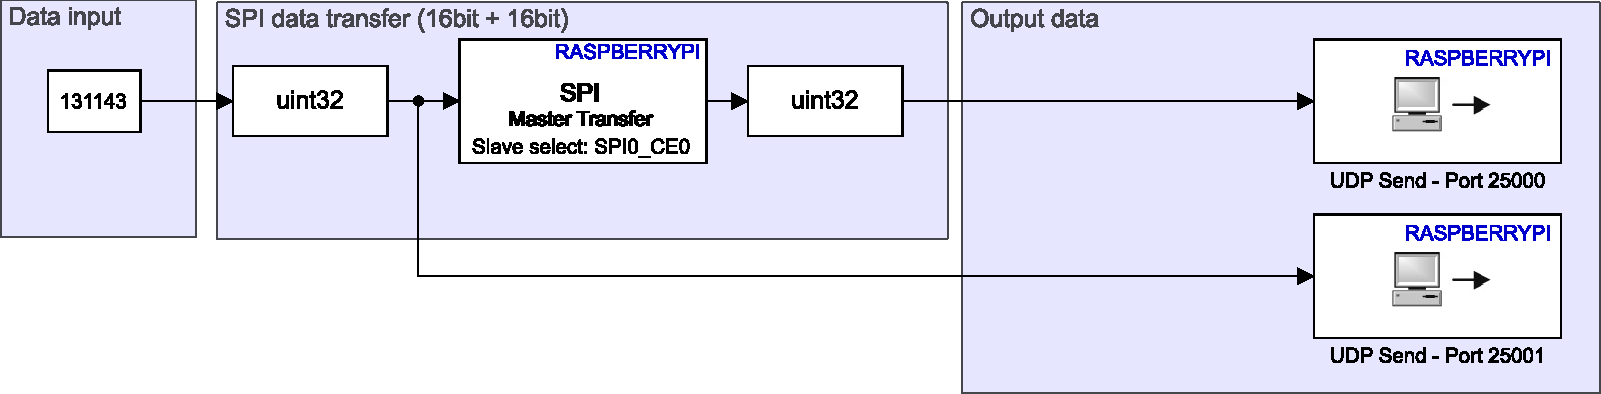
\includegraphics[scale=0.6]{./img/test_raspi_psed_single.pdf}
			\caption{Schema a blocchi simulink implementato}
			\label{fig:simulink_sch}
		\end{figure}

	\section{Configurazione e comunicazione con il Raspberry Pi}
	\label{sec:configurazione_raspberrypi}
			
		Per la creazione di un canale di comunicazione tra \textit{RaspberryPi} e la FPGA \textit{Cyclone III} si è utilizzato il protocollo di comunicazione SPI.

		Di seguito vengono esposti i collegamenti da effettuare sulle due board:

		\begin{table}[ht]
			\centering
			\begin{tabular}{|l|l|}
				\rowcolor{gray!25} % Imposta il colore di sfondo della riga
				\hline
				\textbf{FPGA} & \textbf{Raspberry} \\
				\hline
				GPIO1\_D1 & GPIO8 (CE0) \\
				\hline
				GPIO1\_D3 & GPIO9 (MISO) \\
				\hline
				GPIO1\_D5 & GPIO10 (MOSI) \\
				\hline
				GPIO1\_D7 & GPIO11 (SCK) \\
				\hline
			\end{tabular}
			\caption{Collegamenti pin to pin delle due board}
			\label{tab:wiring}
		\end{table}

		\subsection{Funzionamento della Comunicazione SPI}
		\label{subsec:funzionamento_spi_comm}
			La comunicazione SPI (\textit{Serial Peripheral Interface}) è un protocollo di comunicazione seriale ampiamente utilizzato nell'ambito dell'elettronica embedded. È utilizzato per collegare dispositivi digitali tra loro, consentendo loro di scambiare dati in modo sincrono e affidabile. 

			Il funzionamento della comunicazione SPI si basa su una connessione di tipo master-slave tra dispositivi. In questa configurazione, un dispositivo agisce da "master" e controlla il flusso dei dati, mentre uno o più dispositivi agiscono da "slave" e rispondono alle richieste del master. Il master è responsabile di generare il segnale di clock (SCK) che sincronizza la trasmissione e ricezione dei dati.

			I segnali chiave utilizzati nella comunicazione SPI sono:
			\begin{itemize}
			\item \textbf{SCK (\textit{Serial Clock}):} Questo segnale viene generato dal master e utilizzato per sincronizzare la trasmissione e ricezione dei dati tra i dispositivi. I dati vengono campionati sul fronte di salita o discesa del segnale di clock, a seconda della configurazione.
			
			\item \textbf{MOSI (\textit{Master Output Slave Input}):} Questo è il segnale di uscita del master e di ingresso dello slave. Il master utilizza MOSI per inviare dati agli slave. Quando i dati vengono trasmessi, vengono spostati bit per bit lungo il MOSI, sincronizzati dal segnale di clock.
			
			\item \textbf{MISO (\textit{Master Input Slave Output}):} Questo è il segnale di ingresso del master e di uscita dello slave. Gli slave utilizzano MISO per inviare dati al master. Anche in questo caso, i dati vengono spostati bit per bit lungo il MISO, sincronizzati dal segnale di clock.
			
			\item \textbf{SS/CS (\textit{Slave Select/Chip Select}):} Questo segnale è utilizzato per selezionare uno specifico slave con cui il master vuole comunicare. Il master può avere più linee SS/CS per comunicare con diversi slave. Nel nostro caso indicato come CE0, ovvero \textit{chip enable 0}
			\end{itemize}

			Il funzionamento di una trasmissione SPI inizia quando il master seleziona uno specifico slave mediante il segnale SS/CS. Successivamente, il master inizia a inviare i dati lungo il MOSI, sincronizzati dal segnale di clock SCK. Gli slave campionano i dati in arrivo sul fronte di salita o discesa del segnale di clock e li trasmettono al master tramite il segnale MISO.

			La comunicazione SPI può funzionare sia in modalità full-duplex, in cui il master e lo slave possono trasmettere contemporaneamente, che in modalità half-duplex, in cui la trasmissione avviene in entrambe le direzioni, ma non contemporaneamente.

			Infine, la comunicazione SPI offre un meccanismo efficiente e affidabile per lo scambio di dati tra dispositivi digitali. La sua semplicità e la sua capacità di supportare sia applicazioni a corta distanza che a lunga distanza, ne fanno una scelta ideale per molte applicazioni nell'ambito dell'elettronica e dell'informatica embedded.

\chapter{Risultati sperimentali}
\label{ch:risultati_sperimentali}

	\section{Test eseguiti per valutare le prestazioni del moltiplicatore}
	\label{sec:test_prestazioni}
		\subsection{Risultati ottenuti}
		\label{subsec:risultati}

\chapter{Conclusioni}
\label{ch:conclusioni}

	\section{Principali conclusioni del lavoro svolto}
	\label{sec:conclusioni}
		\subsection{Sviluppi futuri e miglioramenti}
		\label{subsec:sviluppi_futuri}


\end{document}